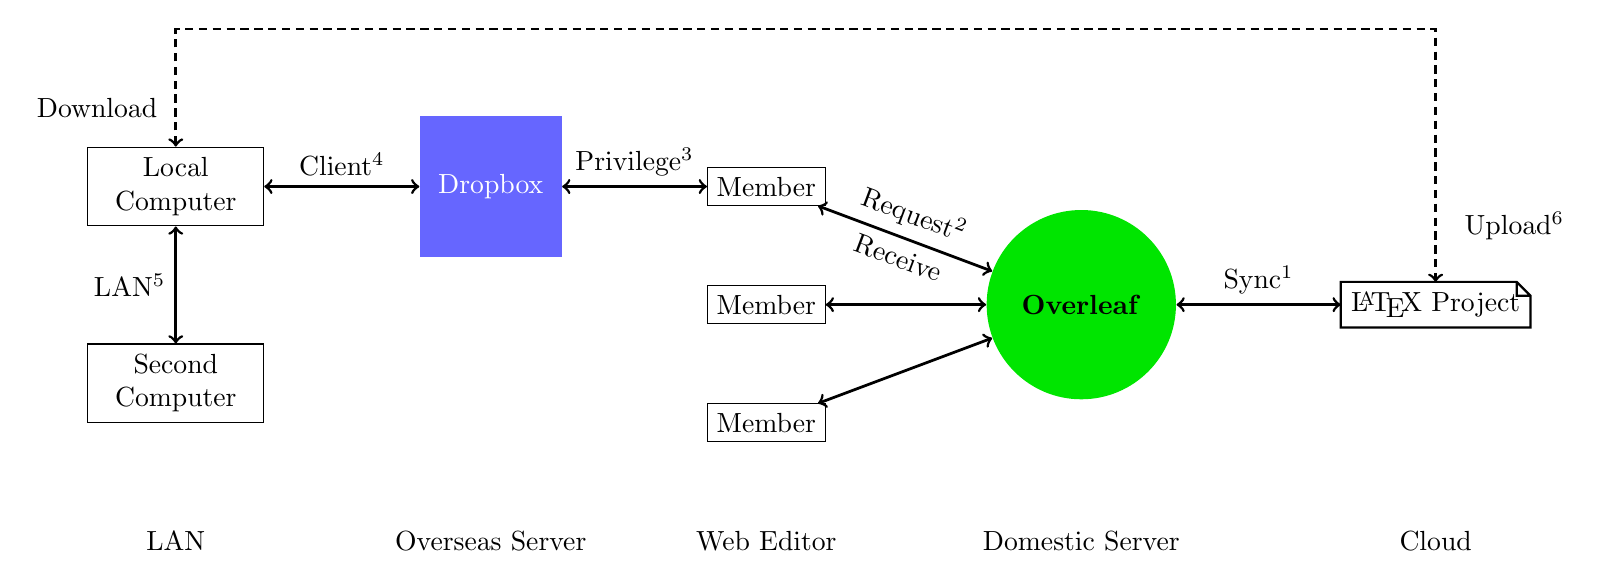
\begin{tikzpicture}

      \makeatletter
      \pgfdeclareshape{document}{
      \inheritsavedanchors[from=rectangle] % this is nearly a rectangle
      \inheritanchorborder[from=rectangle]
      \inheritanchor[from=rectangle]{center}
      \inheritanchor[from=rectangle]{north}
      \inheritanchor[from=rectangle]{south}
      \inheritanchor[from=rectangle]{west}
      \inheritanchor[from=rectangle]{east}
      % ... and possibly more
      \backgroundpath{% this is new
      % store lower right in xa/ya and upper right in xb/yb
      \southwest \pgf@xa=\pgf@x \pgf@ya=\pgf@y
      \northeast \pgf@xb=\pgf@x \pgf@yb=\pgf@y
      % compute corner of ``flipped page''
      \pgf@xc=\pgf@xb \advance\pgf@xc by-5pt % this should be a parameter
      \pgf@yc=\pgf@yb \advance\pgf@yc by-5pt
      % construct main path
      \pgfpathmoveto{\pgfpoint{\pgf@xa}{\pgf@ya}}
      \pgfpathlineto{\pgfpoint{\pgf@xa}{\pgf@yb}}
      \pgfpathlineto{\pgfpoint{\pgf@xc}{\pgf@yb}}
      \pgfpathlineto{\pgfpoint{\pgf@xb}{\pgf@yc}}
      \pgfpathlineto{\pgfpoint{\pgf@xb}{\pgf@ya}}
      \pgfpathclose
      % add little corner
      \pgfpathmoveto{\pgfpoint{\pgf@xc}{\pgf@yb}}
      \pgfpathlineto{\pgfpoint{\pgf@xc}{\pgf@yc}}
      \pgfpathlineto{\pgfpoint{\pgf@xb}{\pgf@yc}}
      \pgfpathlineto{\pgfpoint{\pgf@xc}{\pgf@yc}}
      }
      }
      \tikzstyle{message} = [shape=document, thick, draw=black, minimum width=2cm]
    
\tikzstyle{greencirc} = [circle,fill=green!90!black,inner sep=10];
\tikzstyle{boldarrow} = [<->,line width=1pt];

\node[draw] (v4) at (0,0.5) {Member};
\node[draw] (v1) at (0,-1) {Member};
\node[draw] (v3) at (0,-2.5) {Member};
\node[minimum size=1.8cm,fill=blue!60,text=white] (v6) at (-3.5,0.5) {Dropbox};
\node[greencirc] (v2) at (4,-1) {\textbf{Overleaf}};
\node [message] (v5) at (8.5,-1) {\LaTeX~Project};
\node[text width=2cm,text badly ragged,text centered,draw,minimum size=1cm] (v7) at (-7.5,0.5) {Local Computer};
\node[text width=2cm,text badly ragged,text centered,draw,minimum size=1cm] (v8) at (-7.5,-2) {Second Computer};

\node at (-7.5,-4) {LAN};
\node at (-3.5,-4) {Overseas Server};
\node at (0,-4) {Web Editor};
\node at (4,-4) {Domestic Server};
\node at (8.5,-4) {Cloud};

\draw[boldarrow]  (v1) edge (v2);
\draw [boldarrow] (v3) edge (v2);
\draw [boldarrow] (v4) edge node[above,sloped]{Request$^2$} node[below,sloped]{Receive}(v2);
\draw [boldarrow] (v2) edge node[above] {Sync$^1$}(v5);
\draw [boldarrow]  (v4) edge node[above]{Privilege$^3$}(v6);
\draw [boldarrow] (v6) edge node[above]{Client$^4$}(v7);
\draw [boldarrow] (v7) edge node[left]{LAN$^5$}(v8);

\draw [boldarrow, densely dashed] (v7) -- (-7.5,2.5) -- (8.5,2.5) -- (v5);
\node at (9.5,0) {Upload$^6$};
\node at (-8.5,1.5) {Download};
\end{tikzpicture}